\chapter{Introduction} \label{ch:intro}

The design of a new pharmaceutical treatment for a disease is a complex process involving many stages. Breakthroughs in medical research have enabled a wide variety of different treatment modailities ranging from vaccines to gene therapy, tailored for different diseases - in this thesis, we will narrow our scope to small-molecule drugs, which remain the most common form of treatment for a wide variety of diseases. The development of a new small molecule drug begins with the identification of a target, which is a protein or other biomolecule that plays a role in the disease's biochemical mechanism of action. Afterwards a `hit' compound, which is a small molecule that binds to the target with relatively weak potency, is found as the starting point for a drug design campaign. This brings us to the `hit-to-lead' stage where modifications to the hit are performed to identify a lead compound, which is a small molecule that is potent against the target at very low concentrations. The lead is then optimized to improve its other molecular properties such as target selectivity, solubility, and toxicity. Finally, the lead is taken into preclinical studies and clinical trials to determine its safety and efficacy in humans.

The stages between target identification and preclinical study traditionally follow the design-make-test paradigm, where molecules are repeatedly proposed, synthesized, and assayed. Drug candidates are designed based on some hypothesis relating chemical structure to bioactivity/molecular properties, which gets updated in light of new activity results. This cycle repeats as the molecular search space narrows down until a candidate molecule satisfies the necessary bioactivity/selectivity/toxicity criteria.

The time taken to fully complete a drug design campaign from target identification to preclinical studies can be very time-consuming, costly and there is always a risk of failure if an inappropriate target is chosen or unanticipated side effects are revealed during clinical trials due to the complexity of biology. The costs of developing a new drug have been increasing over time for a multitude of reasons, and there is a pressing need to reduce the time and cost of the drug discovery process.

\begin{figure}[!h] % !h ~ force here, t ~ top, b ~ bottom, p ~ separate page
    \centering
    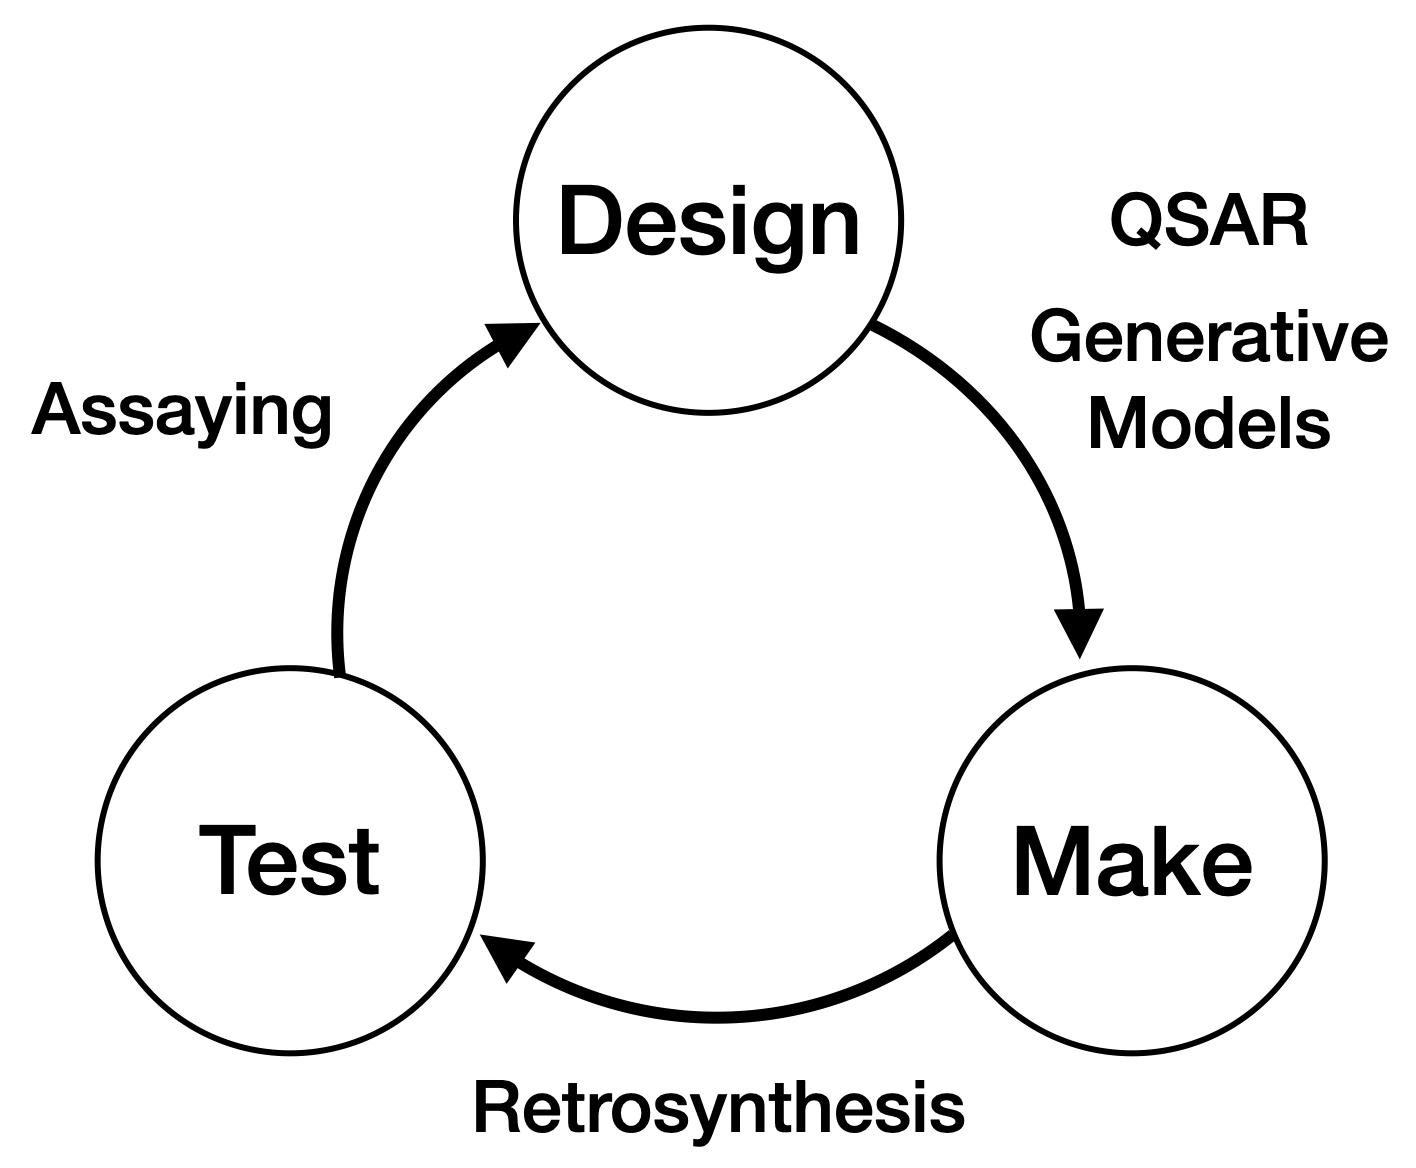
\includegraphics[width=0.5\textwidth]{Chapters/Intro/Figs/design-make-test.png}
    \caption{\label{fig:cycle} An overview of the design-make-test cycle in drug discovery.}
\end{figure}

Computational methods offer a promising avenue to accelerate the drug discovery process by automating the design-make-test cycle. The dream of replacing slow and expensive experiments with fast and cheap predictive algorithms is not a new one, and continuous progress has been made in this direction over the past few decades. Recently, there has been a huge surge in applying machine learning (ML) methods to drug design following its success in various other fields, most notably computer vision and natural language processing.

The application focus for these ML methods have been on the `design' and `make' parts of the cycle, where they have outperformed traditional approaches on a variety of tasks from property prediction to synthesis route planning, and efforts are underway to use ML models to replace aspects of decision-making conventionally done by humans, such as the design of drug candidates.

Much of the progress in this area comes from adapting the latest state-of-the-art algorithms from the ML literature, and while this is a good starting point, it is not sufficient to fully leverage the potential of ML in drug discovery. The quantity and structure of data that is available in drug discovery is very different from that conventionally found in ML applications, and it is necessary to confront this fact and tailor ML models specifically for the unique problems and situations faced in pharmaceutical chemistry in order to drive the development of computational tools that truly suit our needs for accelerating the drug discovery process.

This is the key challenge that we shall explore in this thesis - how we can leverage data-driven approaches based on machine learning in the design-make-test cycle, grappling with the practical difficulties of a drug discovery campaign where we must make full use of the limited data available.

\section*{Design}

The `Design' stage can be broken down into two challenges: (i) predicting the property of a compound from its structure, and (ii) using that predictive model to propose a set of new compounds that are likely to have the desired property. The first challenge has historically been very well-studied: As stated by Alexander Crum Brown in 1868, the ``physiological response of a compound is merely a function of its chemical constitution'' \cite{Brown1868} - chemists have been endeavoring to define this function and predict the properties of compounds without synthesizing them since.

A milestone in the field was made by Hansch and Frujita in 1962 in defining Quantitative Structure-Activity Relationship (QSAR) equations. These were manually defined mathematical models that could be used to predict molecular properties such as the octanol/water partition coefficient (logP) and biological activity, from descriptor coeffiecients derived from molecular structure \cite{hansch1962correlation, hansch1964p}.

Coincidentally, the field of artificial intelligence (AI) was also born in the late 1950s/1960s and the potential of applying computational methods to chemistry was recognized early on with the Dendral system in 1965, which assisted chemists in interpreting mass spectrometry data \cite{Lindsay1993Dendral}. Dendral is not only recognised as the first formal application of AI to chemistry, but also as the first expert system since it was capable of automating some tasks of organic chemists and thereby improving decision making.

Further research into applying AI in chemistry greatly decreased following the general collapse in AI research from the 1970s onwards, and afterwards the workhorse for computational methods in drug design has been in the use of simulations. Advances in computational processing power and the availability of protein-ligand crystal structures led to the development and use of techniques such as molecular docking, molecular dynamics, and free energy perturbation (FEP) \cite{Yu2017CADDMethods}. The success of these methods have cemented the role of computational tools in drug discovery, and they remain in extensive use today.

The breakthoughs of machine learning in other fields such as image recognition and natural language processing in the 21st century has led to a resurgence of interest in applying these methods to drug discovery. The victory of a nerual network model in the Merck molecular activity challenge \cite{Ma2015MerckMolecularActivity} set in motion active research into the application of deep learning for molecular property prediction which continues to this day.

Much of this research consists of translating the latest state-of-the-art algorithms from the ML literature and applying them to the same retrospective QSAR model benchmarks repeatedly to compare performance between different models. While this has undeniable value in quantitatively driving the development of improved models, by focusing only on retrospective benchmarks and avoiding prospective deployment, model developers overlook the unique challenges faced in real-world drug discovery and the practical needs of the end user \cite{Kearnes2021Prospective}.

This thesis addresses this in two places. In Chapter \ref{ch:fresco} we look at how to leverage fragment-protein structures from a crystallographic fragment screen to perform hit discovery in the absence of any bioactivity data via an unsupervised learning approach. Moving onwards to the early hit-to-lead stage, where bioactivity data is limited, noisy, and dominated by inactive molecules, in Chapter \ref{ch:ranking} we use a learning-to-rank framework to make use of inactive data and overcome experimental noise.

Once a predictive model is obtained, the next step of `Design' is to propose a set of new compounds for synthesis and testing. Traditionally this is done by applying the predictive model on a library of compounds (either commercially available or constructed by human experts), and selecting the top scoring compounds. However, this approach is limited by the coverage of the library, and vast chemical space remains unexplored. Generative deep learning models have been proposed as an alternative approach, where a neural network that can generate novel compounds is combined with a predictive model for exploring chemical space. This approach has shown to be successful for several toy problems and offer an interesting alternative to traditional library screening, particularly in the context of intellectual property \cite{Meyers2021DeNovo}. However, even for toy examples it has been shown that imperfections in the predictive model are exploited by the generative model to generate flawed compounds \cite{Renz2019FailureModes}. This is a problem that will be exacerbated in a real world use case, and it is clear that improving predictive modelling of molecular properties is the fundamental bottleneck to successful `Design'.

\section*{Make}
After proposing a set of compounds, the next step is to synthesize them - the central focus of the field of synthetic organic chemistry. Designing a set of chemical reactions that transform a set of starting materials into a target molecule is approached via retrosynthetic analysis, a concept introduced by E.J. Corey \cite{corey1991logic}. In this approach, the target molecule is progressively simplified into  precursor molecules until commercially available compounds are reached. This logical approach paved the way for the successful synthesis of many complex molecules, for which Corey was awarded the Nobel Prize in Chemistry in 1990 \cite{NobelCorey}.

In addition to introducing the concept of retrosynthetic analysis, Corey was also a pioneer in applying computational methods to support the design of synthetic routes \cite{Corey1985ComputerAssistedSynthesis}. By utilising computers to search databases of available compounds as well as previously recorded chemical reactions instead of relying on the necessarily limited experience and domain knowledge of individual chemists, computational tools allowed the design of shorter, more efficient synthesis routes.

Modern-day approaches build on this work, employing deep learning models instead. By taking advantage of vast repostiories of reaction data held in public and propreitary databases as well as ever-growing libraries of commercially available building blocks, ML models for synthesis planning have found significant success in determining synthetic tractability as well as synthesis planning \cite{Coley2018}. Indeed, recent state-of-the-art models have demonstrated their effectiveness through a variation of the Turing test, where computationally designed synthesis routes compete well against those from expert human organic chemists \cite{Coley19WLDN5}.

While there remain limitations on predicting subtle selectivities and reaction yields, it is generally accepted that ML models can accurately predict the major products of reactions that are well-represented in public datasets. This has led to their increasing deployment and use in industry.

However, deep learning-based reaction prediction models critically suffer from a lack of interpretability. Their black-box nature means it is neither clear if the models are making correct predictions because of correct reasoning, nor is it clear what training data and biases they are relying on to reach a prediction \cite{Jimenze2020XAI}. As these models are made more and more available to non-expert end users, it is increasingly important to understand the decision-making of these models in order to avoid incorrect predictions and drive the development of more robust models. To address this, in Chapter \ref{ch:transformer} we showcase a workflow for explaining the reasoning of reaction prediction models.

\section*{Test}
The major focus of machine learning approaches to property prediction has been on improving performance on retrospective datasets, typically involving curated biological activity data obtained from biochemical assays. A great deal of effort is spent on improving molecular representation and the predictive performance of these models, but relatively little thought is given on how this experimental data is generated, and the Test step of the drug discovery process is largely treated as a black box. 

In reality, different biochemical assay techniques have different accuracies and idiosyncracies and the data generated from different assays should not be modelled equally \cite{Hughes2011Principles}. Innovative experimental techniques such as phenotype screening \cite{Chandrasekaran2021Phenotype}, DNA-/Peptide-encoded libraries \cite{GirondaMartinez2021DNALibrary, Rossler2023PeptideLibrary}, and high-throughput spectrometry \cite{Dunas2023MassSpec} are being developed and there are exciting opportunities to apply machine learning methods for the interpretation of these new forms of experimental data.

Beyond just developing ML models to learn this kind of data, there is great potential in engaging with experimentalists to more tightly integrate ML with experimental techniques for the design of ML-centric design-make-test workflows. We explore this in Chapter \ref{ch:testing} where we apply machine learning on crude bioactivity data from nanomolar-scale high-thoughput chemistry.
